%	paper.tex	Toby Searle
%	Last modified: Mon  9 Sep 12:06:19 2013
%	using jfm template

\NeedsTeXFormat{LaTeX2e}

\documentclass{jfm}

\usepackage{graphicx}
\usepackage{natbib}
%%%%%%%%%%%Added to template:
\usepackage{mathtools} % add my own packages
\graphicspath{ {./images/} }
\newcommand\Wi{\mbox{\textit{Wi}}}
%%%%%%%%%%%%%%%

% See if the author has AMS Euler fonts installed: If they have, attempt
% to use the 'upmath' package to provide upright math.
\ifCUPmtlplainloaded \else
  \checkfont{eurm10}
  \iffontfound
    \IfFileExists{upmath.sty}
      {\typeout{^^JFound AMS Euler Roman fonts on the system,
                   using the 'upmath' package.^^J}%
       \usepackage{upmath}}
      {\typeout{^^JFound AMS Euler Roman fonts on the system, but you
                   dont seem to have the}%
       \typeout{'upmath' package installed. JFM.cls can take advantage
                 of these fonts,^^Jif you use 'upmath' package.^^J}%
       \providecommand\upi{\pi}%
      }
  \else
    \providecommand\upi{\pi}%
  \fi
\fi

% See if the author has AMS symbol fonts installed: If they have, attempt
% to use the 'amssymb' package to provide the AMS symbol characters.

\ifCUPmtlplainloaded \else
  \checkfont{msam10}
  \iffontfound
    \IfFileExists{amssymb.sty}
      {\typeout{^^JFound AMS Symbol fonts on the system, using the
                'amssymb' package.^^J}%
       \usepackage{amssymb}%
       \let\le=\leqslant  \let\leq=\leqslant
       \let\ge=\geqslant  \let\geq=\geqslant
      }{}
  \fi
\fi

% See if the author has the AMS 'amsbsy' package installed: If they have,
% use it to provide better bold math support (with \boldsymbol).

\ifCUPmtlplainloaded \else
  \IfFileExists{amsbsy.sty}
    {\typeout{^^JFound the 'amsbsy' package on the system, using it.^^J}%
     \usepackage{amsbsy}}
    {\providecommand\boldsymbol[1]{\mbox{\boldmath $##1$}}}
\fi

%%% Example macros (some are not used in this sample file) %%%

% For units of measure
\newcommand\dynpercm{\nobreak\mbox{$\;$dyn\,cm$^{-1}$}}
\newcommand\cmpermin{\nobreak\mbox{$\;$cm\,min$^{-1}$}}

% Various bold symbols
\providecommand\bnabla{\boldsymbol{\nabla}}
\providecommand\bcdot{\boldsymbol{\cdot}}
\newcommand\biS{\boldsymbol{S}}
\newcommand\etb{\boldsymbol{\eta}}

% For multiletter symbols
\newcommand\Real{\mbox{Re}} % cf plain TeX's \Re and Reynolds number
\newcommand\Imag{\mbox{Im}} % cf plain TeX's \Im
\newcommand\Rey{\mbox{\textit{Re}}}  % Reynolds number
\newcommand\Pran{\mbox{\textit{Pr}}} % Prandtl number, cf TeX's \Pr product
\newcommand\Pen{\mbox{\textit{Pe}}}  % Peclet number
\newcommand\Ai{\mbox{Ai}}            % Airy function
\newcommand\Bi{\mbox{Bi}}            % Airy function

% For sans serif characters:
% The following macros are setup in JFM.cls for sans-serif fonts in text
% and math.  If you use these macros in your article, the required fonts
% will be substitued when you article is typeset by the typesetter.
%
% \textsfi, \mathsfi   : sans-serif slanted
% \textsfb, \mathsfb   : sans-serif bold
% \textsfbi, \mathsfbi : sans-serif bold slanted (doesnt exist in CM fonts)
%
% For san-serif roman use \textsf and \mathsf as normal.
%
\newcommand\ssC{\mathsf{C}}    % for sans serif C
\newcommand\sfsP{\mathsfi{P}}  % for sans serif sloping P
\newcommand\slsQ{\mathsfbi{Q}} % for sans serif bold-sloping Q

% Hat position
\newcommand\hatp{\skew3\hat{p}}      % p with hat
\newcommand\hatR{\skew3\hat{R}}      % R with hat
\newcommand\hatRR{\skew3\hat{\hatR}} % R with 2 hats
\newcommand\doubletildesigma{\skew2\tilde{\skew2\tilde{\Sigma}}}
%       italic Sigma with double tilde

% array strut to make delimiters come out right size both ends
\newsavebox{\astrutbox}
\sbox{\astrutbox}{\rule[-5pt]{0pt}{20pt}}
\newcommand{\astrut}{\usebox{\astrutbox}}

\newcommand\GaPQ{\ensuremath{G_a(P,Q)}}
\newcommand\GsPQ{\ensuremath{G_s(P,Q)}}
\newcommand\p{\ensuremath{\partial}}
\newcommand\tti{\ensuremath{\rightarrow\infty}}
\newcommand\kgd{\ensuremath{k\gamma d}}
\newcommand\shalf{\ensuremath{{\scriptstyle\frac{1}{2}}}}
\newcommand\sh{\ensuremath{^{\shalf}}}
\newcommand\smh{\ensuremath{^{-\shalf}}}
\newcommand\squart{\ensuremath{{\textstyle\frac{1}{4}}}}
\newcommand\thalf{\ensuremath{{\textstyle\frac{1}{2}}}}
\newcommand\Gat{\ensuremath{\widetilde{G_a}}}
\newcommand\ttz{\ensuremath{\rightarrow 0}}
\newcommand\ndq{\ensuremath{\frac{\mbox{$\partial$}}{\mbox{$\partial$} n_q}}}
\newcommand\sumjm{\ensuremath{\sum_{j=1}^{M}}}
\newcommand\pvi{\ensuremath{\int_0^{\infty}%
  \mskip \ifCUPmtlplainloaded -30mu\else -33mu\fi -\quad}}

\newcommand\etal{\mbox{\textit{et al.}}}
\newcommand\etc{etc.\ }
\newcommand\eg{e.g.\ }


\newtheorem{lemma}{Lemma}
\newtheorem{corollary}{Corollary}

\title[Viscoelastic Kelvin-Helmholtz instabilty]{Viscoelastic Kelvin-Helmholtz instability}

\author[T. W. Searle and A. N. Morozov]%
{T. W. Searle$^1$ and A. N. Morozov$^1$%
  \thanks{Email address for correspondence: jfm@damtp.cam.ac.uk},\ns
}

% NOTE: A full address must be provided: department, university/institution, town/city, zipcode/postcode, country.
\affiliation{$^1$SUPA, School of Physics and Astronomy, University of Edinburgh, Mayfield Road,
Edinburgh, EH9 3JZ, UK\\[\affilskip]
}

\pubyear{2013}
\volume{650}
\pagerange{119--126}
% Do not enter received and revised dates. These will be entered by the editorial office.
\date{?; revised ?; accepted ?. - To be entered by editorial office}
%\setcounter{page}{1}
\begin{document}

\maketitle

\begin{abstract}
  Abstract goes here. Abstract goes here. Viscoelastic Kelvin-Helmholtz instability. 
\end{abstract}

\begin{keywords}
Authors should not enter keywords on the manuscript, as these must be chosen by the author during the online submission process and will then be added during the typesetting process (see http://journals.cambridge.org/data/\linebreak[3]relatedlink/jfm-\linebreak[3]keywords.pdf for the full list)
\end{keywords}

\section{Introduction}

Fairly recently, a turbulent state has been discovered in viscoelastic fluids. There is both experimental and theoretical evidence for this. Larson, Shaqfeh and Muller discovered evidence of wavy vortex coherent states in Taylor-Couette flow of a boger viscoelastic fluid at very low Reynolds number \cite{Larson1990}. As well as this numerical and experimental study of Taylor-Couette flow, Groisman and Steinberg \cite{Groisman2000} discovered turbulence in viscoelastic fluids between two counter rotating plates.

For a long time it was thought that the elasticity of a viscoelastic fluid only served to dampen instability. It was observed that the drag in fluid could be reduced by the addition of small amounts of viscoelastic fluid. This drag reduction has been much studied over the last 70 years. However, the studies above give reason to believe that viscoelastic turbulence is present at very low Reynolds number, where it is driven by the elasticity of the polymeric fluid rather than its inertia.

In 1997 Fabian Waleffe identified a Newtonian self sustaining process in plane Couette flow \cite{Waleffe97}. Streamwise rolls redistribute the streamwise velocity into a streaky flow. This streaky flow is unstable through a Kelvin-Helmholtz instability creating a three dimensional perturbation which in turn re-energises the original streamwise rolls. This exact solution to the Navier-Stokes equations is thought to be a component of the transition to turbulence. In 1998 Waleffe constructed a bifurcation diagram for this exact solution \cite{Waleffe98} containing what looks like a bifurcation from infinity. This is the behaviour expected of the transition to turbulence in Couette flow.

Using this work in Newtonian fluid dynamics as a template for the structure of purely elastic turbulence reveals a similar pattern of streaks and, hopefully, a similar self-sustaining process. An important step on the path to explaining this process in purely elastic flows is establishing the mechanism by which the streaks become unstable. Presumably, this will also be a Kelvin-Helmholtz instability as the streaks shear past the rest of the fluid. For this aim we have constructed this simple model system of a shearing viscoelastic fluid.

The Kelvin-Helmholtz instability is fundemental to Newtonian fluids, and is often a source for the transition to turbulence in these fluids. It is hoped that by finding a purely elastic version of this instability, we might be able to probe one of the important mechanisms for the transition to purely elastic turbulence.

We present a linear stability analysis of the Kelvin-Helmholtz instability in the purely elastic regime using direct numerical simulation of both the Oldroyd-B and FENE-CR constituitive models for a polymeric fluid. The purely elastic fluid is found to be unstable at sufficiently high numbers of the dimensionless parameter, the Weissenberg number. The growth rate of the largest growing eigenmode of the instability is found to increase with increasing Weissenberg number for low Weissenberg number. This behaviour is consistent across both the Oldroyd-B and FENE-CR models.

The system we use for our analysis uses a $\tanh$ shaped laminar profile for the streamwise velocity across a plane Couette flow channel, where the instability takes place about $y=0$ as seen in (figure \ref{fig:diagram}). The equation used was:

\begin{align}
    U &= \tanh \left( y/\Delta \right) \coth \left( 1/\Delta \right) \\
    V &= 0 
    \label{eq:KH_laminar_profile}
\end{align}


\begin{figure}
    \centering
    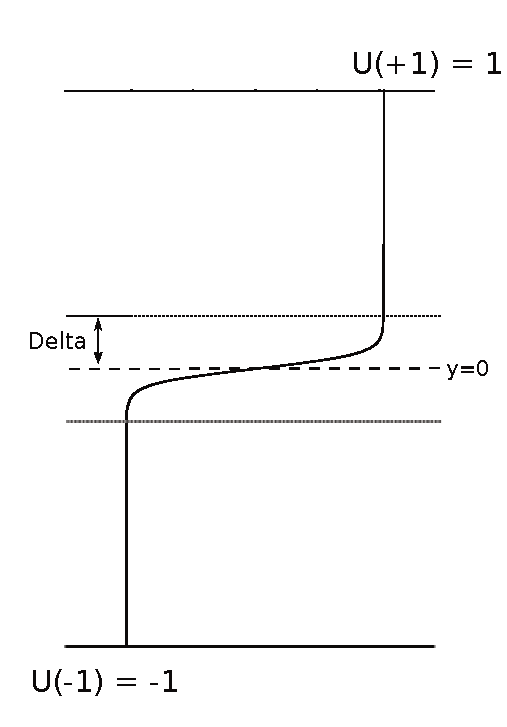
\includegraphics[width=0.6\textwidth]{KH_diagram}
    \caption{diagram of the system}
    \label{fig:diagram}
\end{figure}

\begin{figure}
    \centering
    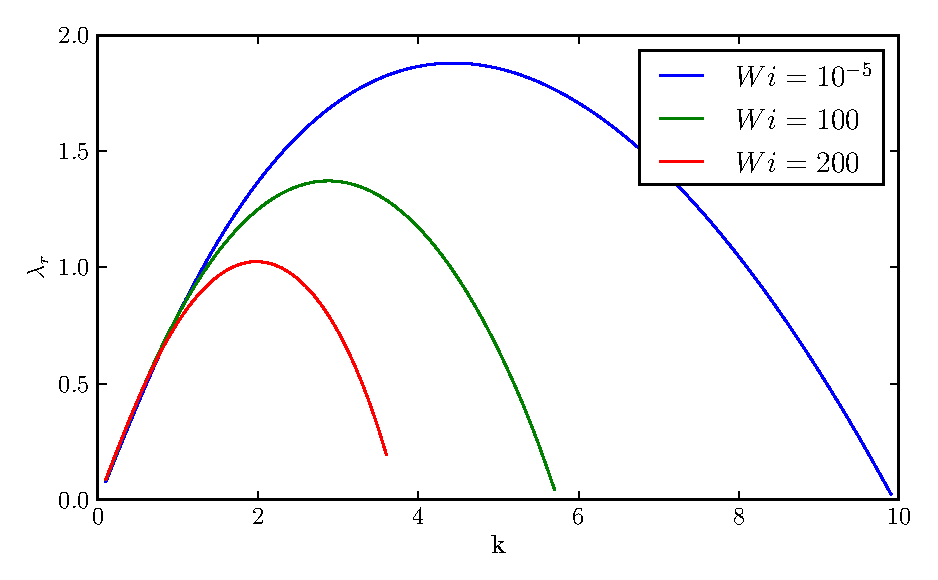
\includegraphics[width=0.5\textwidth]{KH_dispersion}
    \caption{Example of dispersion relation for Weissenberg numbers 200, 100 and $10^{-5}$, with $\beta = 0.1$ and $\Rey = 10000$. Polymer elasticity reduces the height of the instability.}
    \label{fig:KH_growth_rate}
\end{figure}

We performed a Chebyshev decomposition of the flow in the wall-normal ($y$) direction for the base profile, and decomposed the disturbances to this flow in both Chebyshev and Fourier modes.

\begin{equation}
    g(y) = \sum\limits_{m=1}^{m=M} \widetilde{g}_{m} T_{m}(y) e^{ikx + \lambda t}
\end{equation}

for all disturbance variables $g = u, v, p, \tau_{i,j}$. Where $M$ is the number of Chebyshev modes, $T_{m}$ is the mth Chebyshev polynomial of the 1st kind, $k$ is the streamwise wavenumber of the disturbance and $\lambda$ is the growth rate of the mode. 

\section{A purely elastic instability}

For low Reynold's number and high Weissenberg number we see an instability grow from around $k_x \sim 0.1$ and move to lower $k_x$ as the Weissenberg number increases. The height of the instability also increases with increasing Weissenberg number. 

At this point we are unsure as to why the instability is being supressed at high Weissenberg number.

\begin{figure}
    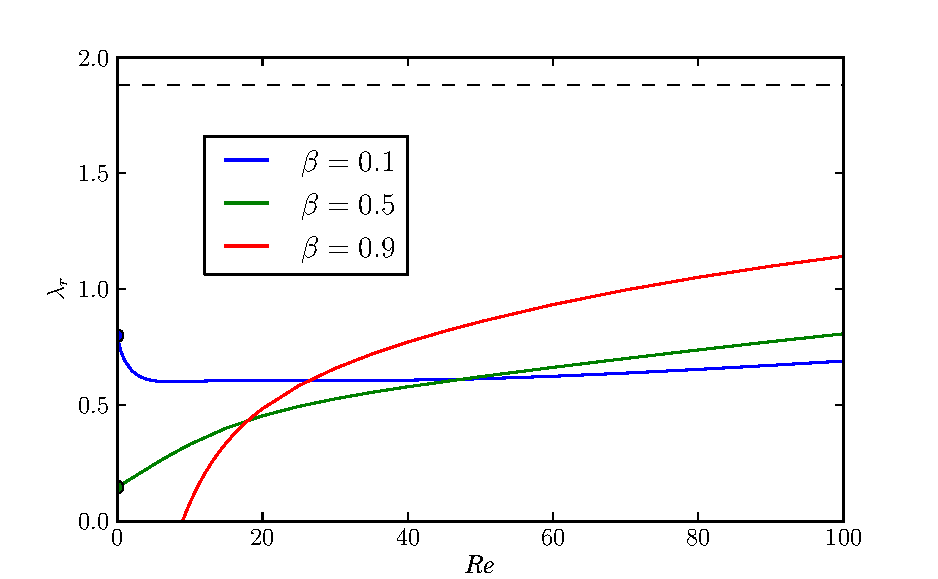
\includegraphics[width=\textwidth]{KH_low_Wi_vary_Re}
    \caption{The change in the height of the dispersion relation as the Reynolds number is reduced at $\Wi=5$. At low $\Rey$ the instability is clearly still present for large polymer concentrations, consistent with purely elastic turbulence. }
    \label{fig:KH_reduce_Re}
\end{figure}
\begin{figure}
    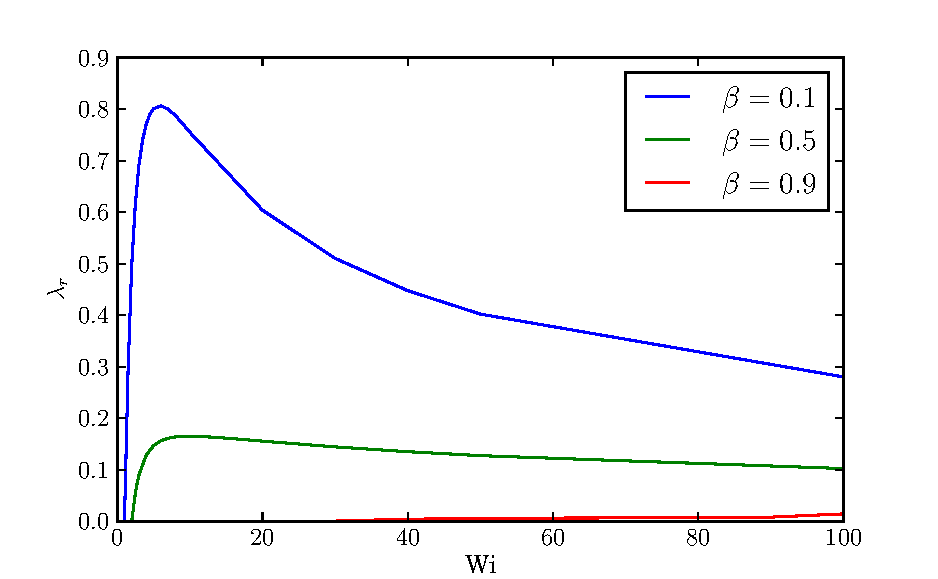
\includegraphics[width=\textwidth]{KH_low_Re_vary_Wi}
    \caption{The change in the height of the dispersion relation as $\Wi$ is increased at $\Rey = 0$. This instability must be entirely elastic in nature. }
    \label{fig:KH_purely_elastic}
\end{figure}
\begin{figure}
    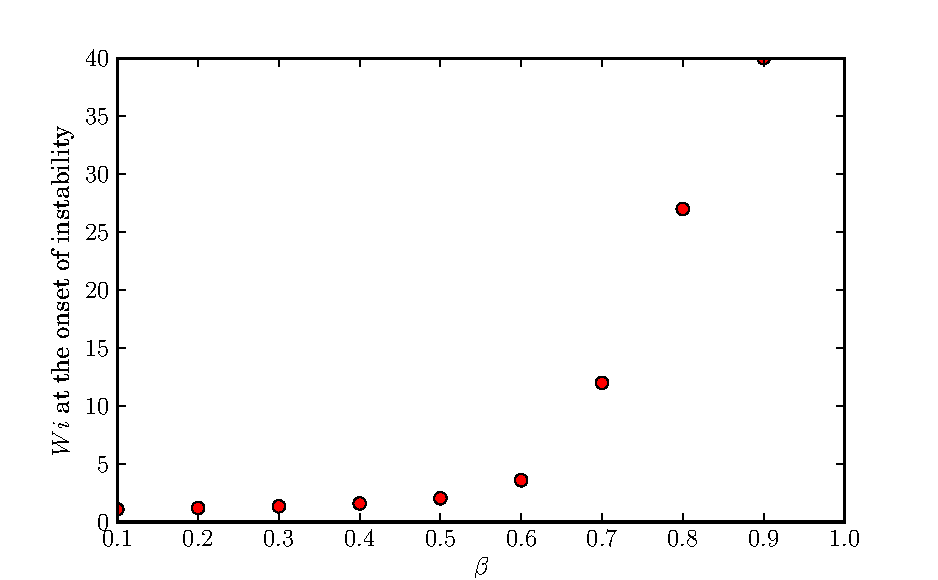
\includegraphics[width=\textwidth]{KH_onset_beta_Wi}
    \caption{The value of the Weissenberg number at which the velocity profile becomes unstable against $\beta$. The onset of the purely elastic instability moves to higher $Wi$ as $\beta$ increases.}
    \label{fig:KH_elastic_onset}
\end{figure}

\section{Confirming the model}

\subsection{Consistency of results with the FENE model}
\begin{figure}
    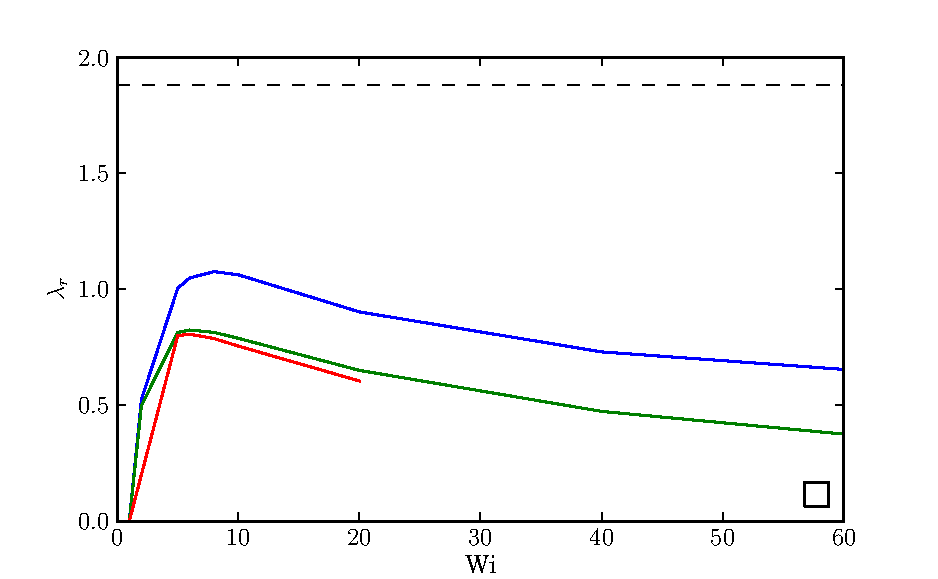
\includegraphics[width=\textwidth]{FENE_low_Re_vary_Wi}
    \caption{Results are consistent with figure \ref{fig:KH_purely_elastic}}
    \label{fig:FENE_low_Re}
\end{figure}


\subsection{Varying width of the instability}

\begin{figure}
    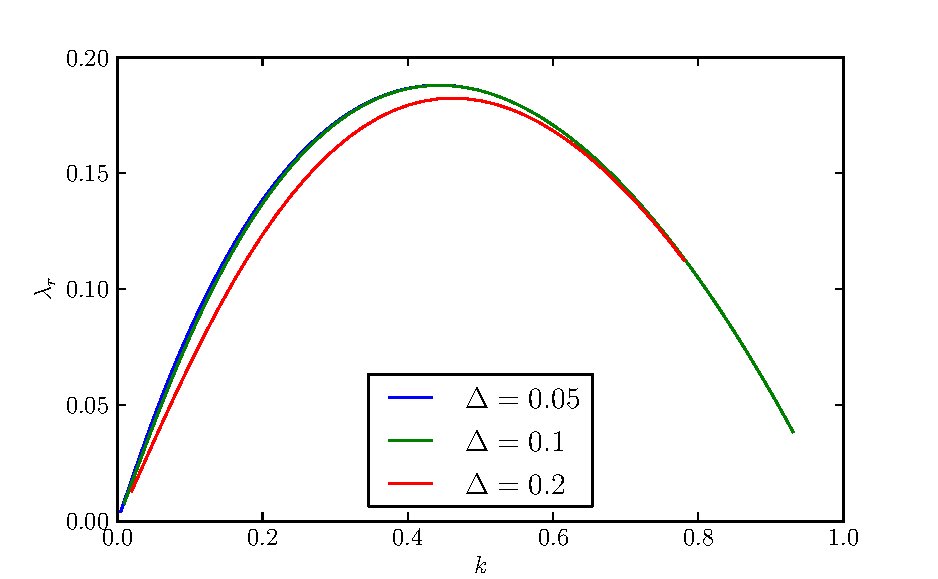
\includegraphics[width=\textwidth]{high_Re_vary_delta}
    \caption{When results are rescaled for the various delta, The instability is found to be insensitive to the width of the instability relative to the wall. At delta = 0.1, $\Rey = 10000$, $\Wi = 0.001$. 300 Gauss-Labatto points were used for each calculation.}
    \label{fig:delta_dispersion}
\end{figure}

\subsection{Drag reduction}

We see drag reduction using the Oldroyd-B model. It is not clear whether or not the maximum drag reduction asymptote is present.



\begin{figure}
%    \showthe\columnwidth %use this to determine size of figures.
    \centering
    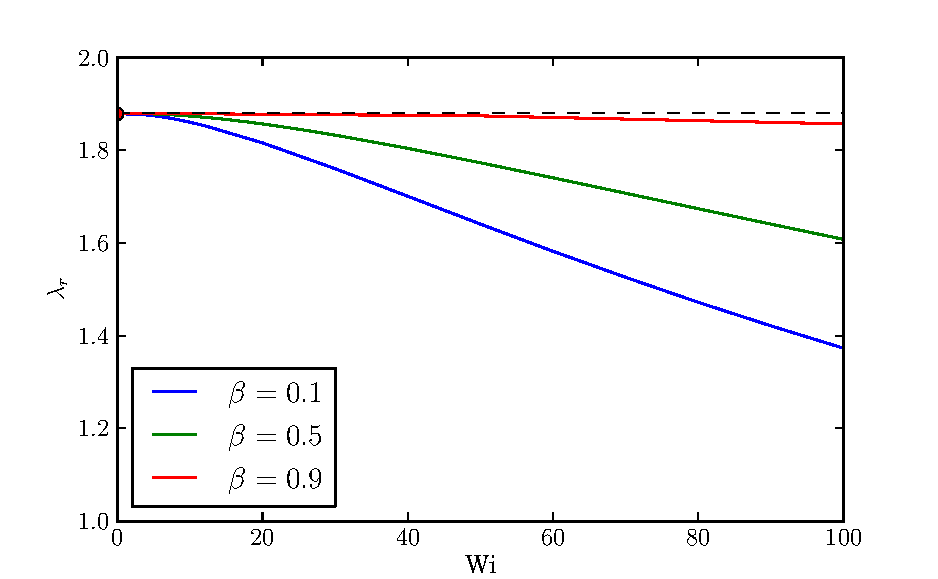
\includegraphics[width=\textwidth]{KH_high_Re_vary_Wi}
    \caption{The height of the dispersion relation is reduced for the Kelvin-Helmholtz instability as the Weissenberg number is increased. The grey dashed line is the height of the dispersion relation for the Newtonian fluid. The decrease in $\lambda_{r}$ corresponds to increased stability of the base flow and so confirms the presence of drag reduction in this system.}
    \label{fig:KH_drag_reduction}
\end{figure}

\section{Conclusions}

What a great and useful thing to have found out. think of all the marvelous implications.

\bibliographystyle{jfm}
% Note the spaces between the initials



%\bibliography{jfm-instructions}

\end{document}
